
\subsection{Что такое видео}

\begin{frame}{Можно ли свести к поиску картинок?}
    \begin{orange-box}{Видео — не картинки}
        \begin{itemize}
            \item $1$ час — $\approx 180 000$  кадров;
            \item искать явно:
            \begin{itemize}
                \item $1$ кадр — $10$ мс;
                \item $1$ видео — $0,5$ часа;
            \end{itemize}
        \end{itemize}
    \end{orange-box}
    \vspace{1em}
    \begin{blue-box}{Видео — не множество}
        \begin{itemize}
            \item есть порядок следования.
        \end{itemize}
    \end{blue-box}
    \vspace{1em}
    \begin{gray-box}{Видео — не текст}
        \begin{itemize}
            \item нужно как-то выбрать символы.
        \end{itemize}
    \end{gray-box}
\end{frame}

\begin{frame}{Можно ли свести к поиску картинок?}
    \begin{grass-green-box}{Нечёткие дубликаты}
        \begin{center}
            \includegraphics[width=\textwidth]{img/video/video-sequence-punctured.pdf}
        \end{center}
    \end{grass-green-box}
    \vspace{1.5em}
    \begin{orange-box}{Совсем разные видео}
        \begin{center}
            \includegraphics[width=\textwidth]{img/video/video-sequence-shuffled.pdf}
        \end{center}
    \end{orange-box}
\end{frame}

\begin{frame}{Можно ли свести к поиску подпоследовательности?}
    \begin{orange-box}{Можно (но не нужно)}
        \begin{center}
            \includegraphics[width=0.9\textwidth]{img/video/video-dna.pdf}
        \end{center}
    \end{orange-box}
\end{frame}

\newcommand{\epath}{./img/video/events}

\newcommand{\eventexample}[1]{
    \includegraphics[width=3.0cm]{\epath/Djadja-Stepa-Milicioner-#1.png}
}


\begin{frame}{Что такое видео: модель представления (1)}
    \begin{center}
        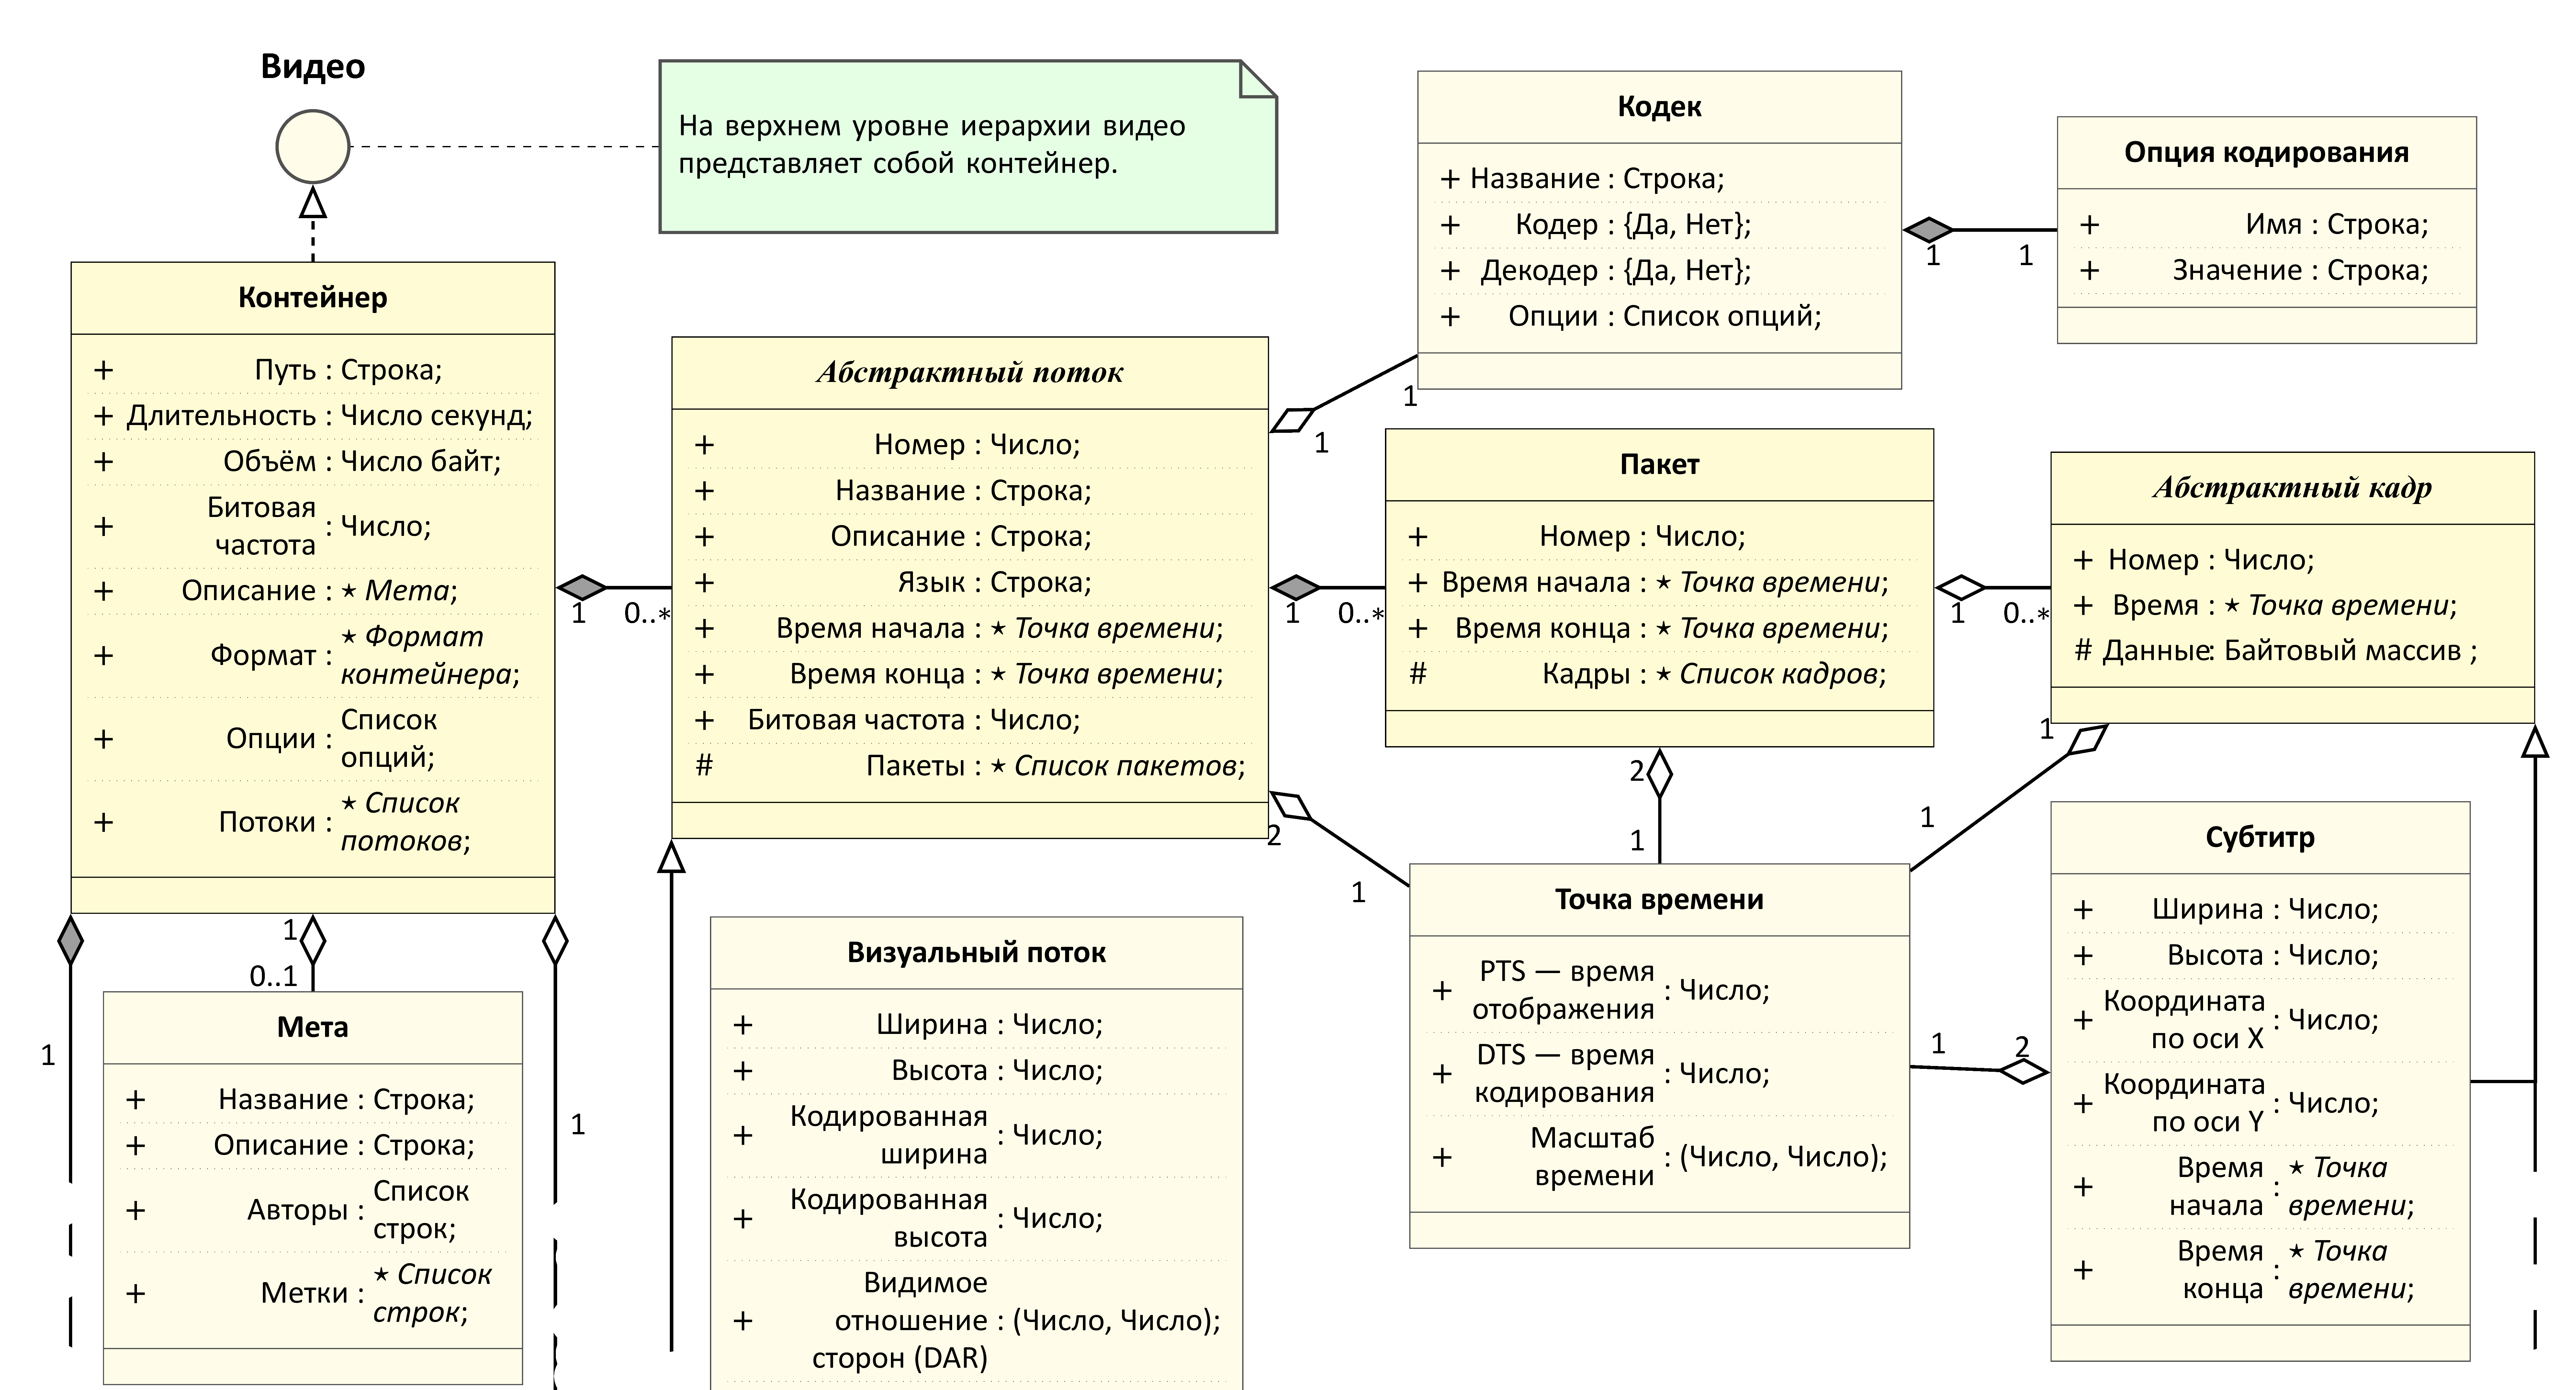
\includegraphics[width=7.5cm]{img/video/video-model-uml-logical.pdf}
    \end{center}
\end{frame}

\begin{frame}{Что такое видео: модель представления (2)}
    \begin{center}
        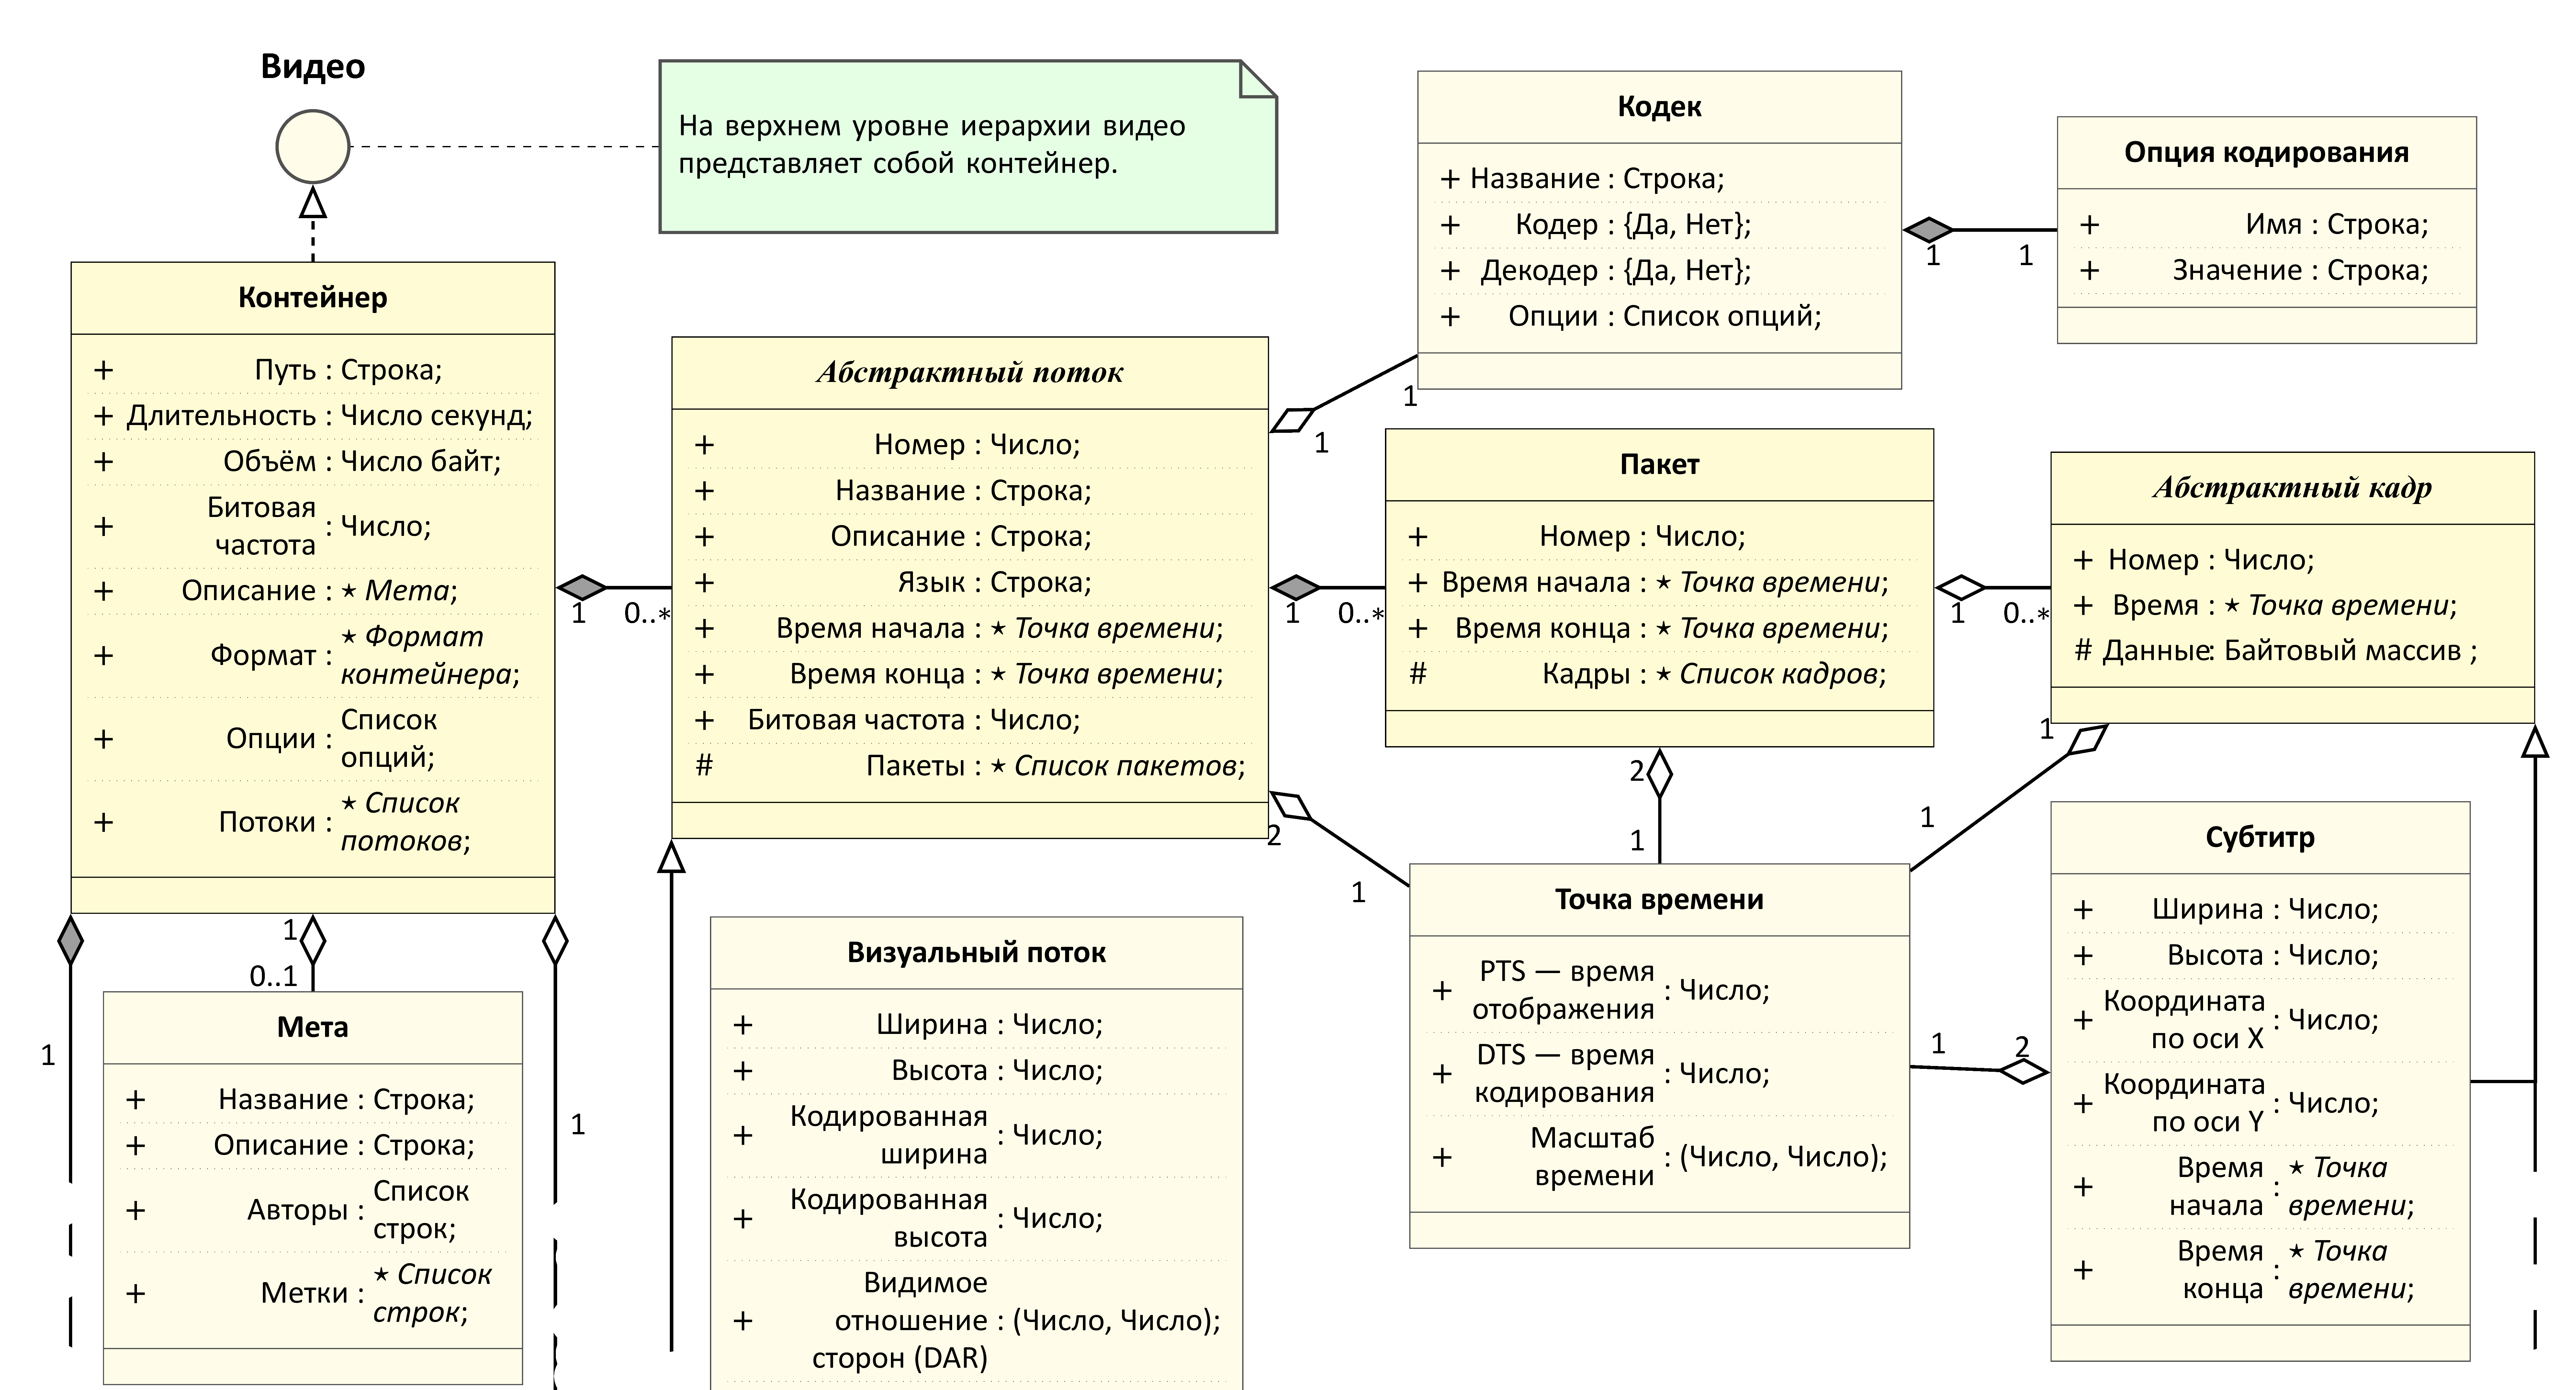
\includegraphics[width=1.05\textwidth]{img/video/video-model-uml-logical.png}
    \end{center}
\end{frame}


\begin{frame}{Что такое видео: концептуальная модель}
    \begin{center}
        \includegraphics[width=8cm]{img/video/video-structure.pdf}
    \end{center}
\end{frame}

\begin{frame}{Что такое видео: логическая модель}
    \begin{center}
        \includegraphics[width=\textwidth]{img/video/video-model-uml-semantic.pdf}
    \end{center}
\end{frame}




% \begin{frame}{Что такое видео?}
%     \begin{gray-box}{Видео — последовательность фактов или событий}
%         \begin{itemize}
%             \item События развиваются во времени.
%             \item Свойства событий
%             — {\it пространственная} характеристика видео,
%             \item продолжительность и порядок фактов — {\it временная}.
%         \end{itemize}%
%     \end{gray-box}
%     \vspace{1.5em}
%     Пример:
%     \begin{center}
%         \begin{tikzcd}[column sep=0.02pc,row sep=0.3pc,ampersand replacement=\&]
%             \raisebox{-.4\height}{\eventexample{1}}
%                  \raisebox{\height}{$\ ;$}
%             \&
%             \raisebox{-.4\height}{\eventexample{2}}
%                  \raisebox{\height}{$\ ;$}
%             \&
%             \raisebox{-.4\height}{\eventexample{3}}
%                   \raisebox{\height}{$\ .$}
%             \\
%         \end{tikzcd}
%         \footnotesize
%         \color{zdarkgreen} 
%         (Кадры событий из начала мультфильма 
%         <<Дядя Стёпа~—~милиционер>>)
%     \end{center}%    
% \end{frame}
